%versi 3 (22-07-2020)
\chapter{Landasan Teori}
\label{chap:teori}

\section{Strategy Pattern}
\label{sec:strategypattern}
~\cite{Gamma:94:design}
Strategy Pattern adalah sebuah design pattern yang memungkinkan objek untuk memilih saat runtime. Ini mendefinisikan sekumpulan algoritma, merangkum masing-masing algoritma, dan membuatnya dapat dipertukarkan. Hal ini memungkinkan klien untuk memilih algoritma berdasarkan kebutuhan mereka tanpa mengubah kode yang menggunakan algoritma tersebut. Ide utama penerapan Strategy Pattern adalah merancang antarmuka fleksibel yang dapat bekerja dengan algoritma berbeda tanpa perlu mengubah kode ketika algoritma baru diperkenalkan. \\
Strategy Pattern cocok digunakan dalam skenario-skenario berikut:
\begin{enumerate}
    \item Ketika ada beberapa kelas terkait yang hanya berbeda dalam perilakunya. Strategy Pattern memungkinkan kelas dikonfigurasikan dengan salah satu dari banyak kemungkinan perilaku.
    \item Ketika ada kebutuhan untuk varian algoritma yang berbeda.
    \item Ketika suatu algoritma melibatkan data yang harus tetap tersembunyi dari klien. Strategy Pattern memastikan bahwa struktur data yang kompleks dan spesifik algoritma tidak terekspos.
    \item Ketika sebuah kelas mendefinisikan banyak perilaku, dan perilaku ini diimplementasikan melalui beberapa pernyataan kondisional. Dalam kasus seperti ini, Strategy Pattern menyederhanakan kode dengan memindahkan cabang kondisional terkait ke dalam kelas Strategi masing-masing
\end{enumerate}
\begin{figure}[h] 
	\centering  
	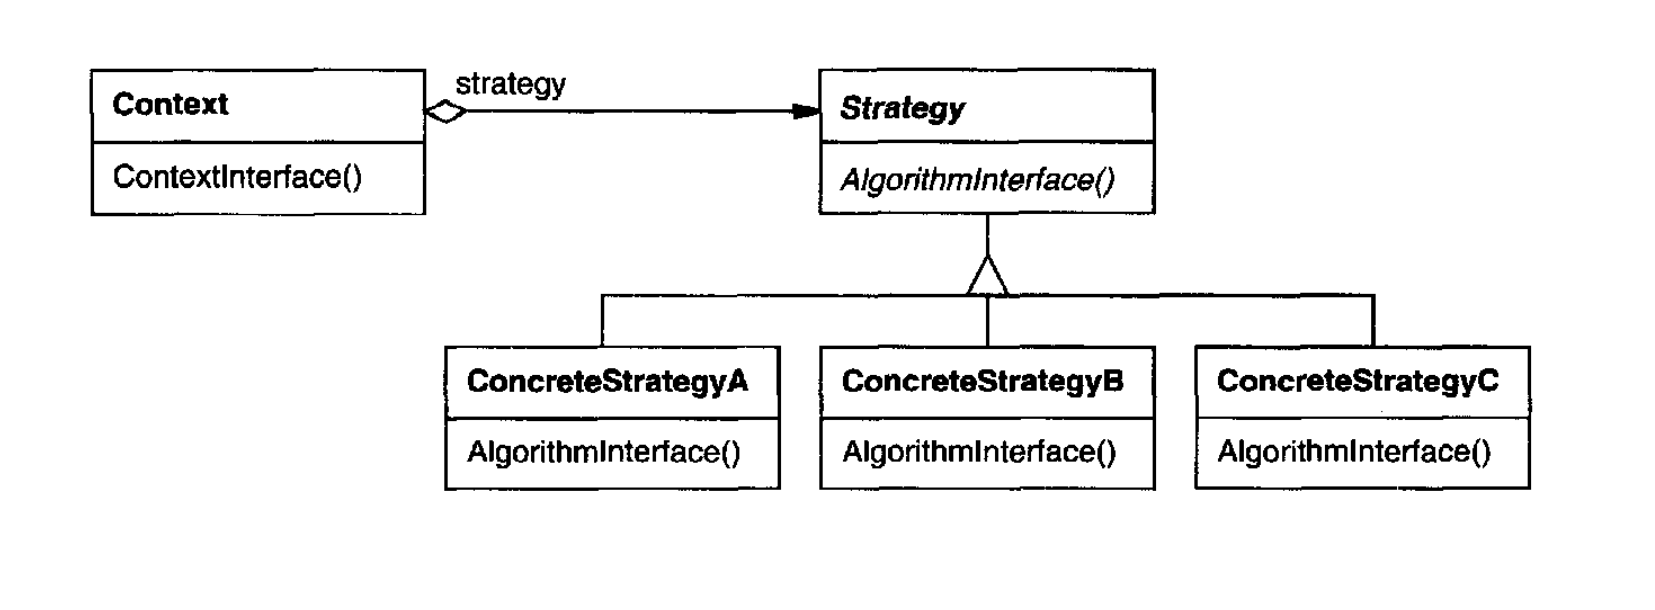
\includegraphics[width=1\textwidth]{struktur-sp}  
	\caption{Struktur Strategy Pattern}
	\label{fig:struktursp} 
\end{figure}

\section{MySQL}
\label{sec:mysql}
MySQL adalah \textit{open source relational database management system} (RDBMS) yang digunakan untuk menyimpan dan mengelola data yang dikembangkan oleh Oracle. MySQL adalah salah satu sistem manajemen basis data paling populer di dunia. SQL adalah singkatan dari \textit{Structured Query Language} yang merupakan bahasa pemrograman yang digunakan untuk mengambil, memperbarui, menghapus, dan memanipulasi data dalam database relasional. Sebagai database relasional, MySQL menyimpan data dalam tabel baris dan kolom yang disusun dalam skema. Skema mendefinisikan bagaimana data diatur dan disimpan serta menjelaskan hubungan antara berbagai tabel. \\
Manfaat utama MySQL meliputi hal berikut:
\begin{itemize}
    \item \textbf{\textit{Ease Of use}}. Pengembang dapat menginstal MySQL dengan mudah, dan database mudah dikelola.
    \item \textbf{\textit{Reliability}}. MySQL adalah salah satu database yang paling matang dan banyak digunakan. Teknologi ini telah diuji dalam berbagai skenario selama hampir 30 tahun, termasuk oleh banyak perusahaan terbesar di dunia.
    \item \textbf{\textit{Scalability}}. MySQL berskala untuk memenuhi permintaan aplikasi yang paling banyak diakses. Arsitektur replikasi asli MySQL memungkinkan organisasi, termasuk Facebook, Netflix, dan Uber, meningkatkan aplikasi untuk mendukung puluhan juta pengguna atau lebih.
    \item \textbf{\textit{Performance}}. MySQL adalah sistem database tanpa administrasi yang terbukti berkinerja tinggi dan hadir dalam berbagai edisi untuk memenuhi hampir semua permintaan.
    \item \textbf{\textit{High availability}}. MySQL menghadirkan serangkaian teknologi replikasi asli dan terintegrasi penuh untuk ketersediaan tinggi.
    \item \textbf{\textit{Security}}. Keamanan data mencakup perlindungan data dan kepatuhan terhadap peraturan industri dan pemerintah.
    \item \textbf{\textit{Flexibility}}. Penyimpanan Dokumen MySQL memberi pengguna fleksibilitas maksimum dalam mengembangkan aplikasi database tradisional bebas skema SQL dan NoSQL.
\end{itemize}

\subsection{LineString}
\label{subs:linestring}
Di MySQL, LineString adalah tipe data spasial yang digunakan untuk merepresentasikan geometri linier, seperti jalur atau garis, dalam ruang dua dimensi. MySQL menyediakan berbagai fungsi spasial untuk bekerja dengan geometri LINESTRING, termasuk mengukur panjangnya, menentukan perpotongannya, dan banyak lagi. Fitur-fitur ini sangat berguna dalam aplikasi Sistem Informasi Geografis (GIS) dimana data spasial seperti jalan atau sungai perlu disimpan dan dianalisis. \\
Format untuk mendefinisikan LINESTRING adalah sebagai berikut: \\
\texttt{LINESTRING(x1 y1, x2 y2, x3 y3, ...)}

\newpage

\section{Algoritma Dijkstra}
\label{sec:dijkstra}
~\cite{Cormen:09:intro}
Algoritma Dijkstra menyelesaikan masalah \textit{single-source shortest path}, yaitu menemukan jalur terpendek dari satu titik asal ke semua titik lainnya dalam sebuah graf berarah dengan bobot tepi non-negatif. Proses ini dimulai dengan menginisialisasi perkiraan jarak terpendek dari titik asal $s$ ke semua titik lain. Jarak titik asal sendiri diatur ke nol, sedangkan titik lainnya diatur sebagai tak hingga. Algoritma ini menggunakan sebuah struktur \textit{min-priority queue} (antrean prioritas minimum) yang menyimpan titik-titik dengan prioritas sesuai dengan perkiraan jarak terpendek mereka dari titik asal.
\\
Selama eksekusi, algoritma Dijkstra akan secara bertahap memindahkan titik dengan estimasi jarak terpendek dari antrean ke dalam satu set $S$, yang menampung titik-titik dengan jarak terpendek yang sudah final. Untuk setiap titik $u$ yang baru dipindahkan ke dalam set $S$, algoritma akan memeriksa setiap tetangganya $v$ dan memperbarui perkiraan jarak terpendek ke $v$ jika melalui $u$ memberikan jarak yang lebih pendek. Proses ini dikenal sebagai “relaksasi” tepi, yaitu memperbarui perkiraan jarak dan menunjuk $u$ sebagai pendahulu $v$ bila ditemukan jalur yang lebih optimal.
\\
Proses algoritma berlanjut hingga semua titik di graf telah diproses, sehingga jarak terpendek dari titik asal $s$ ke setiap titik yang dapat dijangkau sudah final. Kompleksitas waktu dari algoritma ini bergantung pada implementasi antrean prioritas yang digunakan, dengan menggunakan \textit{Fibonacci heap}, algoritma Dijkstra dapat mencapai kompleksitas $O(VlogV+E)$, yang efisien untuk graf yang jarang (sparse). Algoritma ini sangat bermanfaat dalam berbagai aplikasi yang melibatkan pencarian jalur terpendek, seperti sistem navigasi dan perutean jaringan.

\section{Algoritma Floyd-Warshall}
\label{floydwarshall}
~\cite{Cormen:09:intro}
Algoritma Floyd-Warshall menyelesaikan masalah jalur terpendek untuk semua pasangan titik dalam graf berarah dengan menggunakan pendekatan pemrograman dinamis. Algoritma ini sangat berguna untuk graf yang memiliki bobot sisi negatif, selama tidak terdapat siklus dengan bobot negatif dalam graf tersebut. Pendekatan ini menghitung jalur terpendek antara semua pasangan titik dengan menggunakan tabel bobot antar titik dan mengulanginya secara bertahap untuk mencapai solusi optimal.
\\
Langkah pertama dalam algoritma ini adalah mempersiapkan matriks bobot jalur terpendek yang akan terus diperbarui. Algoritma memulai dengan menganggap setiap titik memiliki jalur langsung ke dirinya sendiri dengan bobot nol, sementara bobot antar titik lain mengikuti nilai bobot sisi pada graf. Secara rekursif, algoritma memperbarui jalur terpendek dengan menambahkan titik perantara secara bertahap, yaitu jika titik $k$ menjadi perantara dari titik $i$ ke $j$, maka bobot jalur terpendek $d_{ij}$ akan diperbarui menjadi minimum dari $d_{ij}$ atau $d_{ik} + d_{kj}$. Proses ini mengoptimalkan semua jalur antara pasangan titik dengan menambahkan satu titik perantara setiap kali iterasi dilakukan.
\\
Algoritma Floyd-Warshall memiliki kompleksitas waktu $O(V^3)$ karena terdiri dari tiga lapisan perulangan untuk semua titik dalam graf, dengan V sebagai jumlah titik. Meskipun kompleksitasnya tinggi, algoritma ini cukup praktis untuk graf ukuran sedang dan memiliki struktur yang sederhana sehingga dapat diimplementasikan secara efisien. Selain itu, hasil algoritma ini dapat digunakan untuk mendeteksi siklus dengan bobot negatif dalam graf, jika ada nilai negatif pada diagonal utama dari matriks akhir, maka graf tersebut memiliki siklus negatif.
\\
Algoritma ini juga memungkinkan pencarian jalur terpendek melalui matriks pendahulu yang mencatat titik sebelumnya pada jalur terpendek untuk setiap pasangan titik. Dengan matriks ini, jalur terpendek antara titik manapun dapat direkonstruksi secara efisien.

\section{Algoritma A*}
\label{a*}
~\cite{Russell:09:ai}
Algoritma A* adalah metode pencarian yang meminimalkan estimasi total biaya solusi dengan menggabungkan dua fungsi, yaitu  
$g(n)$ dan $h(n)$ Fungsi $g(n)$ menghitung biaya aktual dari titik awal hingga simpul $n$, sedangkan $h(n)$ memperkirakan biaya tersisa dari $n$ ke tujuan. Kombinasi ini menghasilkan $f(n) = g(n) + h(n)$, yang memberikan perkiraan total biaya solusi jika rute melalui simpul $n$. Algoritma ini biasanya dipilih karena dapat mencapai solusi yang optimal dan lengkap, terutama jika fungsi heuristik $h(n)$ memenuhi kriteria tertentu.
\\
Kondisi utama yang diperlukan agar A* memberikan solusi optimal adalah heuristik $h(n)$ yang bersifat \textit{admissible}, yaitu tidak pernah melebih-lebihkan biaya ke tujuan, dan \textit{consistent} atau \textit{monotonic}, di mana nilai $h$ tidak menurun di sepanjang jalur. Dengan adanya heuristik yang memenuhi syarat ini, A* dapat menghindari eksplorasi simpul-simpul yang tidak relevan, mengurangi waktu dan memori yang dibutuhkan.
\\
Terdapat kendala utama dari algoritma A*, yaitu penggunaan memori yang besar karena algoritma ini perlu menyimpan semua simpul yang telah dihasilkan. Meskipun waktu komputasi dapat diatasi dengan baik, kebutuhan memori yang tinggi sering kali menjadi tantangan. Untuk mengatasi hal ini, terdapat varian A* seperti \textit{Iterative-Deepening A*} (IDA*) yang mengurangi kebutuhan memori tanpa mengorbankan optimalitas solusi, dengan biaya eksekusi yang sedikit lebih tinggi.